% !TEX TS-program = pdflatexmk
\documentclass[12pt]{amsart}

%\usepackage[parfill]{parskip}    % Activate to begin paragraphs with an empty line rather than an indent

\usepackage[margin=1in]{geometry}

\usepackage{amsmath,amssymb,amsthm,latexsym,graphicx}
\usepackage[normalem]{ulem}
\usepackage{setspace} %used for doublespacing, etc.
\usepackage{hyperref}
\usepackage{cancel}
\usepackage[dvipsnames,usenames]{color}
\usepackage[all]{xy}
\usepackage{fancyhdr}
\pagestyle{fancy}
	\renewcommand{\headrulewidth}{0.5pt} % and the line
	\headsep=1cm
	
\DeclareGraphicsRule{.tif}{png}{.png}{`convert #1 `dirname #1`/`basename #1 .tif`.png}

%Some useful environments.
\newtheorem{theorem}{Theorem}
\newtheorem{corollary}[theorem]{Corollary}
\newtheorem{conjecture}[theorem]{Conjecture}
\newtheorem{lemma}[theorem]{Lemma}
\newtheorem{proposition}[theorem]{Proposition}
\newtheorem{definition}[theorem]{Definition}
\newtheorem{example}[theorem]{Example}
\newtheorem{axiom}{Axiom}
\theoremstyle{remark}
\newtheorem{remark}{Remark}
\newtheorem*{exercise}{Exercise}%[section]

%Some shortcuts helpful for our assignments
\newcommand{\bx}{\begin{exercise}}
\newcommand{\ex}{\end{exercise}}

%Some useful shortcuts for our favorite sets of numbers.
%Note, you can use these WITHOUT entering math mode
\def\RR{\ensuremath{\mathbb R}} 
\def\NN{\ensuremath{\mathbb N}}
\def\ZZ{\ensuremath{\mathbb Z}}
\def\QQ{{\ensuremath\mathbb Q}}
\def\CC{\ensuremath{\mathbb C}}
\def\EE{{\ensuremath\mathbb E}}

%Some useful shortcuts for formatting lists
\newcommand{\bc}{\begin{center}}
\newcommand{\ec}{\end{center}}
\newcommand{\be}{\begin{enumerate}}
\newcommand{\ee}{\end{enumerate}}
\newcommand{\bi}{\begin{itemize}}
\newcommand{\ei}{\end{itemize}}

%Some useful shortcuts for formatting mathematical symbols
\newcommand{\ol}[1]{\overline{#1}}
\newcommand{\oimp}[1]{\overset{#1}{\iff}} %labeled iff symbol
\newcommand{\bv}[1]{\ensuremath{ \vec{\mathbf{#1}}} } %makes a vector.
\newcommand{\mc}[1]{\ensuremath{\mathcal{#1}}} %put something in caligraphic font
\newcommand{\normale}{\trianglelefteq}
\newcommand{\normal}{\triangleleft}

%Code for formatting the proofs a little nicer for submitted homework
\makeatletter
\renewenvironment{proof}[1][\proofname]{\par\doublespacing
  \pushQED{\qed}%
  \normalfont \topsep6\p@\@plus6\p@\relax
  \list{}{%
    \settowidth{\leftmargin}{\itshape\proofname:\hskip\labelsep}%
    \setlength{\labelwidth}{0pt}%
    \setlength{\itemindent}{-\leftmargin}%
  }%
  \item[\hskip\labelsep\itshape#1\@addpunct{:}]\ignorespaces
}{%
  \popQED\endlist\@endpefalse
  \singlespacing
}
\makeatother

%Commenting tools for the professor
\newcommand{\mpg}[1]{\marginpar{ #1}} %to put comments in margins
\usepackage{soul}
\definecolor{highlight}{rgb}{1,0.6,0.6}
\sethlcolor{highlight}
\newcommand{\hlm}[1]{\colorbox{highlight}{$\displaystyle #1$}}
\newtheoremstyle{mycomment}{\topsep}{-0in}{\small \itshape \sffamily}{}{\small \itshape\sffamily}{:}{.5em}{}
\theoremstyle{mycomment}
\newtheorem*{acomment}{\color{BrickRed}{Comment}}
\newcommand{\com}[1]{{\color{OliveGreen}\begin{acomment}{#1} %#2 \color{black} 
\end{acomment}\noindent}}
\newcommand{\red}[1]{{\color{BrickRed} #1}}
\newcommand{\blue}[1]{{\color{MidnightBlue}#1}}
\newcommand{\green}[1]{{\color{OliveGreen}#1}}
\newcommand{\mwrong}[2]{\red{\cancel{#1}}\green{#2}}
\newcommand{\wrong}[2]{\red{\sout{#1}}\green{#2}}
\definecolor{OliveGreen}{rgb}{.3,.5,.2}
\definecolor{MidnightBlue}{rgb}{.3,.4,.6}
\newcommand{\pts}[1]{\hfill\blue{{#1}/5}}

\chead{MATH 265F}
\pagestyle{fancy}
%Modify these items:
\rhead{\emph{Your Full Name Here}}
\lhead{\emph{HW \#11}}

\begin{document}

\thispagestyle{fancy}

\section*{Section 11.1} 

\begin{exercise}[5] Here is a digram for a relation $R$ on a set $A$. Write the sets $A$ and $R$.
\centering{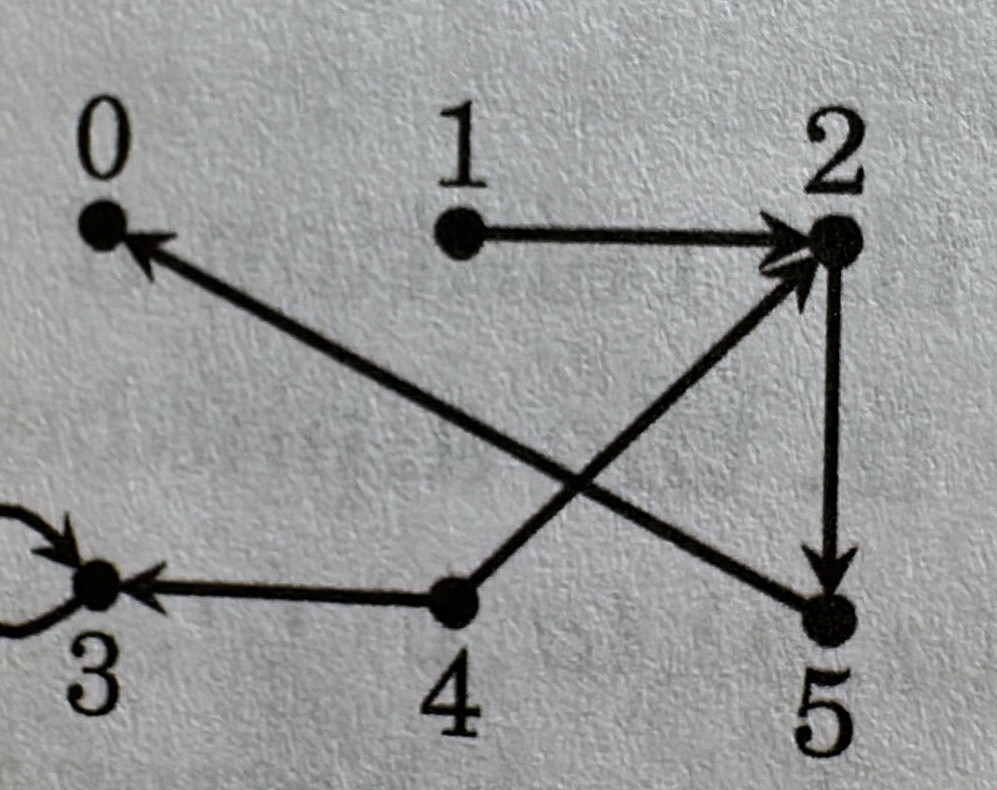
\includegraphics[height=1in]{11p1p5.jpg}}
\begin{proof}[Solution]

\end{proof}
\end{exercise}
\begin{exercise}[6] Congruence modulo 5 is a relation on the set $A=\ZZ$. In this relation $xRy$ $x\equiv y\pmod 5$. Write out the set $R$ in set-builder notation.
\begin{proof}[Solution]
Write your answer here.
\end{proof}
\end{exercise}

In the following exercises, subsets $R$ of $\RR^{2}$ or $\ZZ^{2}$ are indicated by gray shading. In each case, $R$ is a familiar relation on $\RR$ or $\ZZ$. State it.
\begin{exercise}[12] 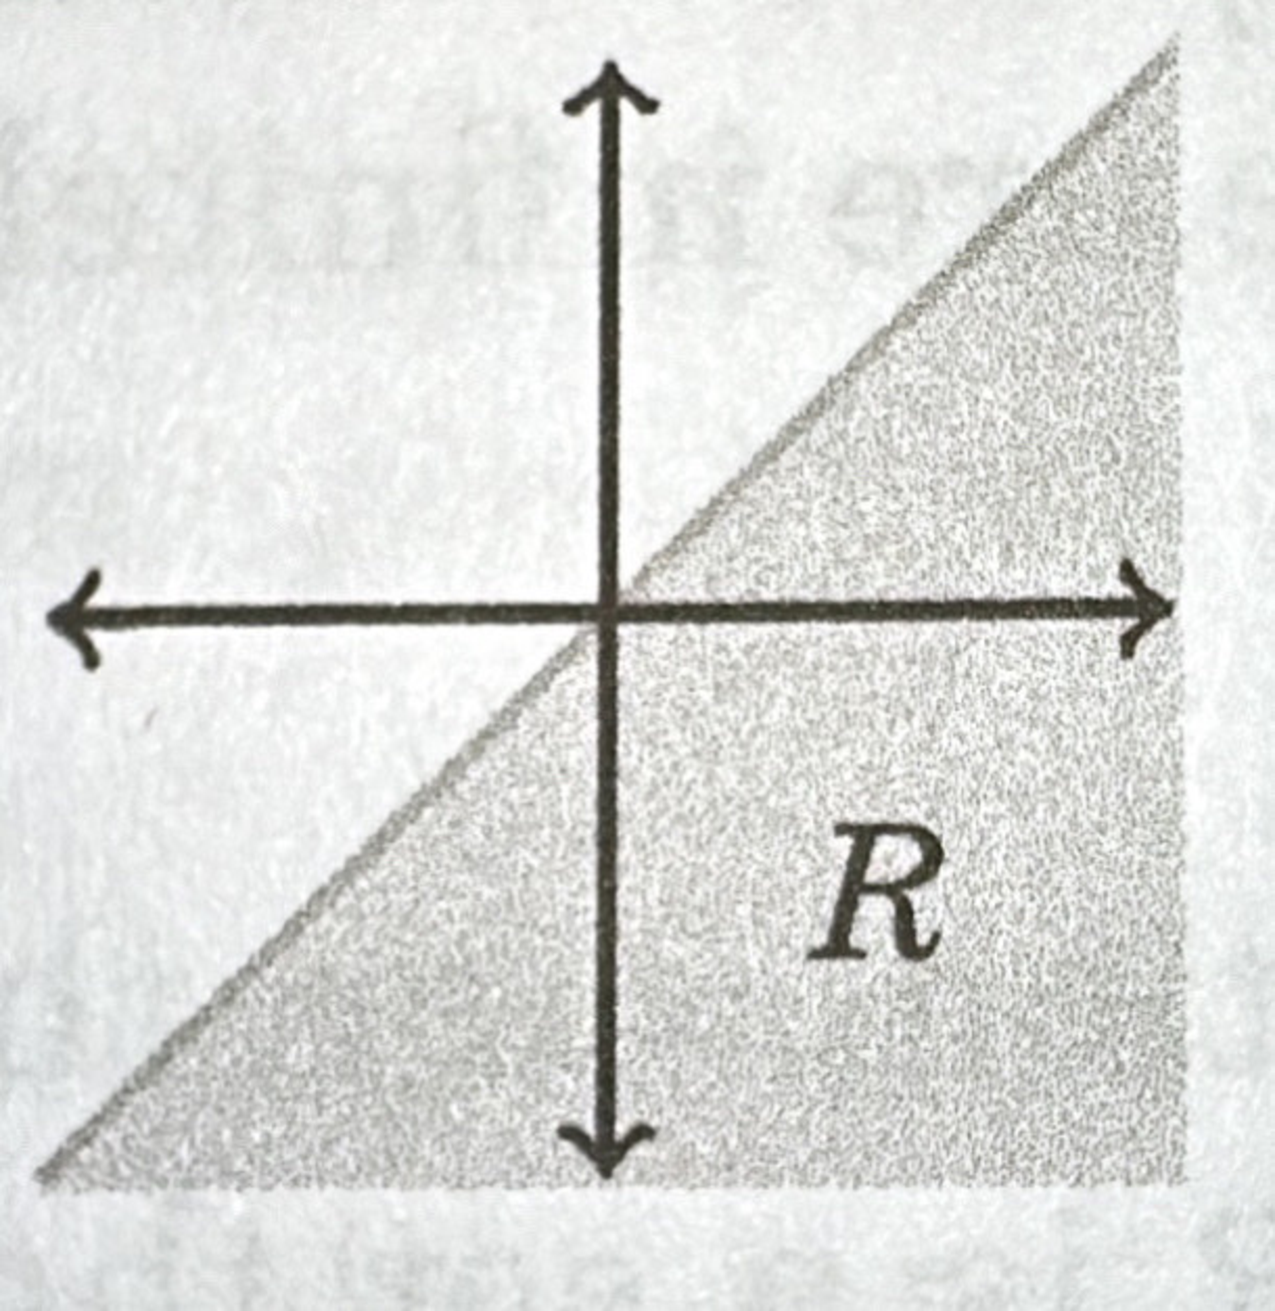
\includegraphics[width=1in]{11p1p12.pdf}
\begin{proof}
Write your answer here.
\end{proof}
\end{exercise}
\section*{Section 11.2}
\emph{Note: When a property does not hold, it suffices to describe {\bf a} counterexample.}
\begin{exercise}[2] Consider the relation $R=\{(a,b),(a,c),(c,c),(b,b),(c,b), (b,c)\}$ on the set $A=\{a,b,c\}$. Is $R$ reflexive? Symmetric? Transitive? If a property does not hold, say why.
\begin{proof}[Solution]
Write your answer here.
\end{proof}
\end{exercise}

\begin{exercise}[5] Consider the relation $R=\{(0,0),(\sqrt{2},0),(0,\sqrt[2]),(\sqrt{2},\sqrt{2})$ on $\RR$. Is $R$ reflexive? Symmetric? Transitive? If a property does not hold, say why.
\begin{proof}[Solution]
Write your answer here.
\end{proof}
\end{exercise}

\begin{exercise}[6] Consider the relation $R=\{(x,x):x\in\ZZ\}$ on \ZZ. Is $R$ reflexive? Symmetric? Transitive? If a property does not hold, say why.
\begin{proof}[Solution]
Write your answer here.
\end{proof}
\end{exercise}

\begin{exercise}[8] Define a relation on \ZZ as $xRy$ if $|x-y|<1$. Is $R$ reflexive? Symmetric? Transitive? If a property does not hold, say why. What familiar relation is this?
\begin{proof}[Solution]
Write your answer here.
\end{proof}
\end{exercise}

\begin{exercise}[12] Prove that the relation $|$ (divides) on the set \ZZ is reflexive and transitive. (Use example 11.8 as a guide if you are unsure how to proceed.)
\begin{proof}[Solution]
Write your answer here.
\end{proof}
\end{exercise}

\begin{exercise}[14] Suppose $R$ is a symmetric and transitive relation on a set $A$, and there is an element $a\in A$ for which $aRx$ for every $x\in A$. Prove that $R$ is reflexive.
\begin{proof}
Write your answer here.
\end{proof}
\end{exercise}

\begin{exercise}[15] Prove or disprove: If a relation is symmetric and transitive, then it is also reflexive.
\begin{proof}[Solution]
Write your answer here.
\end{proof}
\end{exercise}

\section*{Section 11.3}

\begin{exercise}[3] Let $A=\{a,b,c,d,e\}$. Suppose $R$ is an equivalence relation on $A$. Suppose $R$ has three equivalence classes. Also $aRd$ and $bRc$. Write out $R$ as a set.
\begin{proof}[Solution]
Write your answer here.
\end{proof}
\end{exercise}

\begin{exercise}[5] There are two different equivalence relations on the set $A=\{a,b\}$. Describe them. Diagrams will suffice.
\begin{proof}[Solution]
Write your answer here.
\end{proof}
\end{exercise}

\begin{exercise}[8] Define a relation $R$ on \ZZ as $xRy$ iff $x^{2}+y^{2}$ is even. Prove $R$ is an equivalence relation. Describe its equivalence classes.
\begin{proof}
Write your answer here.
\end{proof}
\begin{proof}[Solution]
Write your answer here.
\end{proof}
\end{exercise}



\section*{Section 11.4}
\begin{exercise}[1] List all the partitions of the set $A=\{a,b\}$. Compare your answer to the answer to Exercise 5 of Section 11.3.
\begin{proof}[Solution]
Write your answer here.
\end{proof}
\end{exercise}

\begin{exercise}[4] Suppose $P$ is a partition of a set $A$. Define a relation $R$ on $A$ by declaring $xRy$ if and only if $x,y\in X$ for some $X\in P$. Prove that $R$ is an equivalence relation on $A$. Then prove that $P$ is the set of equivalence classes of $R$.
\begin{proof}
Write your answer here.
\end{proof}
\end{exercise}

\begin{exercise}[Reflection Problem] \ 
\begin{itemize}
\item How long did it take you to complete each problem? 
\begin{proof}[Answer]
\end{proof}
\item What was easy?
\begin{proof}[Answer]
\end{proof}
\item What was challenging? What made it challenging?
\begin{proof}[Answer]
\end{proof}
\item Compare your answers to the odd numbered exercises to those in the back of the textbook. What did you learn from this comparison?
\begin{proof}[Answer]
\end{proof}
\end{itemize}
\end{exercise}.















 \end{document} 